\section{SRResCGAN}

\begin{frame}{Idea}
    对于有先验的影像超分问题建模为:
    \begin{equation*}
        \hat{E}(X) = arg \min\nolimits_{X} \frac{1}{2}\parallel Y-HX \parallel_{2}^{2} + \lambda R_{W}(X)
    \end{equation*}
    作者经过一些列复杂推导得到:
    \begin{equation*}
        X = P_{C}(H^{T}Y-\alpha \sum_{k=1}^{K} L_{k}^{T}\Phi_{K}(L_{k}Y))
    \end{equation*}
    作者根据上式设计了生成器的模型. 例如$\Phi_{K}$在模型中为$PReLU$和残差结构的设计等.
\end{frame}

\begin{frame}{Model}
    在LR数据制作部分, 直接使用DownsampleGAN, 得到具有自然图像高频信息的LR数据集. 
    \begin{figure}
        \centering
        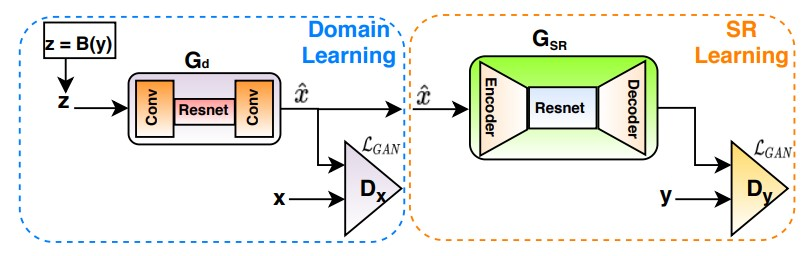
\includegraphics[height=3.5cm]{pic/pic0201.jpg}
        \caption{SRResCGAN模型}
        \label{fig:0201}
    \end{figure}
\end{frame}

\begin{frame}{Loss Function}
    \[ L_{G_{SR}} = L_{per} + L_{tex} + L_{tv} + 10\cdot L_{1} \]
    \begin{itemize}
        \item $L_{per}$人眼感知信息
        \item $L_{tex}$关注高频信息
        \item $L_{tv}$关注梯度差异, 可以更好产生细节信息
        \item $L_{1}$整体差异
    \end{itemize}
\end{frame}